
\section{Projektplanung}

Zum einen wurden in der Projektplanung, die Termine und die zu bearbeitenden Arbeiten definiert und zum anderen wurde eine Risikobwertung durchgeführt.


\subsection{Projektplan}

Die Termine wurde anhand der vorgegebenen Abgabetermine definiert.
Da es vier Abgabetermine gibt, wurde das Projekt in vier Sprints aufgeteilt, die jeweils mit einem Meilenstein enden.

Die folgende Abbildung \ref{fig:roadmap} zeigt die Roadmap mit den definierten Meilstensteinen. Die Meilensteine sind die einzelnen Testatabgaben.
Die abzugebenden Dokumente pro Testat bilden die einzelnen Sprintziele.

\begin{figure}[H]
\centering
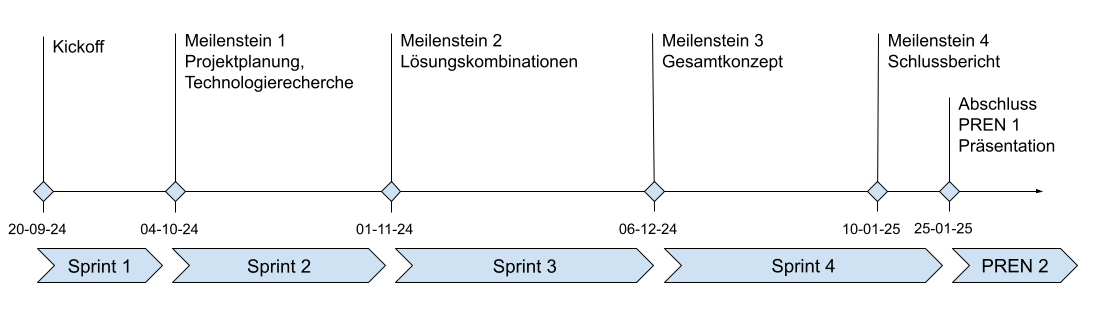
\includegraphics[width=\textwidth]{img/projektplan.png}
\caption{Roadmap}
\label{fig:roadmap}
\end{figure}

Der Projektstrukturplan in Tabelle \ref{table:projektplan} beschreibt die Meilensteine, die zu erreichen sind, detailliert.

\begin{table}[H]
\centering
\begin{tabular}{|l  l l|}
\hline
  \textbf{Meilenstein} & \textbf{Datum} & \textbf{Beschreibung} \\
  \hline
  Meilenstein 1  & 04. Oktober 2024 & \makecell{Projektplan, Skizzierung der Aufgabenstellung,\\ Technologierecherche, Anforderungsliste}\\
  \hline
  Meilenstein 2  & 01. November 2024 & \makecell{Evaluation der Lösungsprinzipien, Auswahl der\\ optimalen Lösungeskombinationen}\\
  \hline
  Meilenstein 3  & 06. Dezember 2024 & \makecell{Freigabe des Gesamtkonzepts, Simulator Wegplanung, \\Dokumentation zu 80\% fertiggstellt}\\
  \hline
  Meilenstein 4  & 10. Januar 2025 & \makecell{Schlussbericht, Präsentation}\\
  \hline
\end{tabular}
\caption{Projektplan}
\label{table:projektplan}
\end{table}

\subsection{Backlog}

Der Backlog dient als zentrales Planungselement.
In diesem Projekt sind die einzelnen Meilensteine vorgegeben. Aus diesem Grund wurden bereits zu Beginn alle Sprints geplant und der ganze Product Backlog wurde in Sprintbacklogs aufgeteilt. Nach Erreichen eines Meilensteins wird ein Ausblick auf den nächsten Sprint durchgeführt, um allfällige Anpassungen an dem Sprintbacklog vorzunehmen.

\subsection{Sprintplanung}

In den folgenden Kapiteln wurden für jeden Sprint Sprintziele definiert und ein Sprintbacklog erstellt. Für den Sprintbacklog wurden die einzelnen Meilensteine aus dem Projektplan in Epics\footnote{https://www.atlassian.com/agile/project-management/epics} beschrieben. Zu den Epics wurden User Stories erstellt. Der Aufwand der einzelnen Stories wurde mit T-Shirt Grössen geschätzt. Die einzelnen T-Shirt Grössen werden wie folgt in eine Zeitdauer umgerechnet:

\begin{table}[H]
\centering
\begin{tabularx}\textwidth{|X | X |}
\hline
  \textbf{Grösse} & \textbf{Dauer} \\
  \hline
  S  & 4h - 2d \\
  \hline
  M  & 2d - 5d\\
  \hline
  L  & 5d+\\
  \hline
\end{tabularx}
\caption{T-Shirt Grössen}
\label{table:t-shirt}
\end{table}


\newpage
\subsubsection{Sprint 1: 20. September 2024 - 04. Oktober 2024}

\textbf{Sprintziel:}
\begin{itemize}
    \item Projektplan erstellt
    \item Aufgabenstellung skizziert
    \item Andorderungsliste erstellt
    \item Technologierecherche
\end{itemize}

\textbf{Sprintbacklog:} Der Sprintbacklog von Sprint 1 ist in Tabelle \ref{table:sprint1-backlog} dargestellt.

\begin{table}[H]
\centering
\small
\begin{tabularx}{\textwidth}{|l|l|X|c|}
\hline
  \textbf{Nr.} & \textbf{Titel} & \textbf{Beschreibung} & \textbf{Size}\\
  \hline
  1  & \textbf{Projektorganisation definieren} &&\\
  \hline
  1.1  & Rollendefinition & Die Rollen Projektleiter und Werkstattverwantwortliche werden definiert. & S\\
  \hline
  1.2 & Datenaustausch definieren & Zentrale Datenablage und Kommunikationsschnittstellen definieren.& S\\
  \hline
  1.3 & Ziele definieren & Definieren, wie wir uns den Roboter vorstellen. & S\\
  \hline
  1.4 & Vorgehen definieren & Geeignete Projektmethode wird gewählt. & S\\
  \hline
    1.5 & Risikomatrix erstellen & Risiken werden gesammelt und bewertet. & M\\
  \hline
  2 & \textbf{Aufgabenstellung klären} && \\
  \hline
  2.1 & Anforderungsliste erstellen & Anforderungen, die der Roboter erfüllen muss sammeln& M \\
  \hline
  2.2 & Aufgabenstellung skizzieren & Modellierunge der Aufgabe zum Verständnis. & S \\
  \hline
  3 & \textbf{Projektplanung} && \\
  \hline
  3.1 & Projektplan erstellen & Meilensteine definieren. & S \\
  \hline
  3.2 & Backlog erstellen & Product Backlog für alle Sprints erstellen. & M \\
  \hline
  4 & \textbf{Lösungsvarianten erarbeiten} && \\
  \hline
  4.1 & Teilfunktionen finden & Roboter in Teilfunktionen aufteilen & S \\
  \hline
  4.2 & Technologierecherche & Recherche zu den einzelnen Teilfunktionen  durchführen. & L\\
  \hline
 
\end{tabularx}
\caption{Sprint 1 Backlog}
\label{table:sprint1-backlog}
\end{table}

\textbf{Sprintreview}

Alle definierten Ziele wurden erreicht. Die geplanten Dokumente wurden erstellt und in einem Entwurf des Schlussberichts eingefügt.

\textbf{Sprint Retrospektive}

Die Zusammenarbeit ist sehr gut gelungen. Die Kennenlernphase war recht kurz und alle Teammitglieder konnten schon früh offen miteinander kommunizieren. Die grösste Herausforderung war die Zeit. Der erste Sprint dauerte lediglich zwei Wochen, jedoch sollte eine ausführliche Technologierecherche durchgeführt werden, die die Basis der weiteren Arbeiten bildet.

\textbf{Risikoupdate}

Im ersten Sprint wurde die Risikoanalyse erstellt. Diese kann im Kapitel Risikobewertung \ref{risk} eingesehen werden.

\newpage
\subsubsection{Sprint 2: 04. Oktober 2024 - 01. November 2024}

\textbf{Sprintziel:}
\begin{itemize}
    \item Evaluation der Lösungsprinzipien
    \item Auswahl der optimalen Lösungeskombinationen
\end{itemize}

\textbf{Sprintbacklog:} Der Sprintbacklog von Sprint 2 ist in Tabelle \ref{table:sprint2-backlog} dargestellt.


\begin{table}[H]
\centering
\small
\begin{tabularx}{\textwidth}{|l|l|X|c|}
\hline
  \textbf{Nr.} & \textbf{Titel} & \textbf{Beschreibung} & \textbf{Size}\\
  \hline
  1  & \textbf{Evaluation Lösungsvarianten} &&\\
  \hline
  1.1  & Workshop Auschlusskriterien & Brainstorming, um herauszufinden, was wir nicht wollen, um Technologien auszuschliessen. & S\\
  \hline
  1.2 & Erste Aussortierung & Lösungsvarianten aussortieren ahhand Auschlusskriterien. & M\\
  \hline
  1.3 & Morphologischer Kasten & Morphologischer Kasten erstellen, um Lösungskombinationen zu ermitteln. & L\\
  \hline
  1.4 & Nutzwertanalyse & Nutzwertanalyse durchführen, um passendste Lösungskombinationen zu ermitteln. & L\\
  \hline
  2 & \textbf{Simulator} && \\
  \hline
  2.1 & Entwicklungsumgebung & Entwicklungsumgebung erstellen. & S \\
  \hline
  2.2 & Konzept erarbeiten & Konzept des Simulators definieren analog zu der Evaluation der anderen Lösungsvarianten. & M \\
  \hline
  2.3 & Wegfindung implementieren & Wegfindung in einem Graphen implementieren. & M \\
  \hline

\end{tabularx}
\caption{Sprint 2 Backlog}
\label{table:sprint2-backlog}
\end{table}

\textbf{Sprintreview}

Alle definierten Ziele wurden erreicht mithilfe von morphologischen Kasten und Nutzwertanalysen. Ebenfalls konnte mit der Entwicklung des Simulators begonnen werden.

\textbf{Sprint Retrospektive}

In diesem Sprint war der Zeitdruck weniger hoch. Dadurch konnte bereits mit ersten Gedanken zum Protoypen begonnen werden, obwohl dies noch nicht eingeplant war, was die Stimmung im Team verbesserte.

\textbf{Risikoupdate}

In diesem Sprint kam das Risiko 7: Ein Objekt wird fehlerhaft gedeutet und falsche Wege werden intern entfernt hinzu. Dies wurde erstellt nach ersten Tests mit Bilderkennungssoftwares. Es wurde dabei festgestellt, dass der Boden in der Mensa stark spiegelt und Erkennung von Knoten und somit der genaue Standort der Hindernisse erschwert.

\newpage
\subsubsection{Sprint 3: 01. November 2024 - 06. Dezember 2024}

\textbf{Sprintziel:}
\begin{itemize}
    \item Dokumentation ist zu 80\% fertiggestellt
    \item Freigabe des Gesamtkonzepts
\end{itemize}

\textbf{Sprintbacklog:} Der Sprintbacklog von Sprint 2 ist in Tabelle \ref{table:sprint2-backlog} dargestellt.

\begin{table}[H]
\centering
\small
\begin{tabularx}{\textwidth}{|l|l|X|c|}
\hline
  \textbf{Nr.} & \textbf{Titel} & \textbf{Beschreibung} & \textbf{Size}\\
  \hline
  1  & \textbf{Gesamtkonzept} & Gesamtkonzept wird mittels Prototyping ausgearbeitet.&\\
  \hline
  1.1  & Konzept Chassis (M) &  Das Konzept der Form wird definiert. & M\\
  \hline
  1.2  & Konzept Fortbewegung \& Lenkung (M) &  Das Konzept der Fortbewegung wird definiert. & M\\
  \hline
  1.3 & Konzept Hindernisse bewegen (M) & Es wird definiert, wie Hindernisse bewegt werden sollen. & L\\
  \hline
  1.4 & Konzept Linienerkennung (ET) & Die Linienerkennung wird definiert. & M\\
  \hline
  1.5 & Konzept Antriebe (ET) & Der Antrieb und wie dieser angesteuert wird wird definiert. & M\\
  \hline
  1.6 & Konzept Objekterkennung (ET) & Es wird definiert, wie Objekte erkannt werden. & L\\
  \hline
  1.7 & Konzept Steuerung (ET/I) & Es wird definiert, wie der Roboter gesteuert wird. & L\\
  \hline
    1.8 & Konzept Wegfindung (I) & Es wird definiert, wie der Weg, den der Roboter gehen soll, ausgewählt wird.  & M\\
\hline
    1.9 & Konzept Bilderkennung (I) & Es wird definiert, wie das Wegenetzwerk und die Hindernisse erkannt werden. & L\\
\hline
    1.10 & Konzept \acrfull{i/o} (M/ET/I) & Es wird definiert, wie das Ziel ausgewählt wird und wie kommuniziert wird, dass der Roboter am Ziel angekommen ist. & M\\
\hline

  2  & \textbf{Simulator} &&\\
  \hline
    2.1 & Hinderniserkennung & Implementieren, dass Hindernisse erkannt und unterschieden werden. Die Reaktion ist je nach Hindernis anders.& M \\
    \hline
  
\end{tabularx}
\caption{Sprint 3 Backlog}
\label{table:sprint3-backlog}
\end{table}

\textbf{Sprintreview}

Alle definierten Ziele wurden erreicht. Dazu konnte bereits zu jeder Story mit Prototyping begonnen werden, jedoch sind einige Teilbereiche noch in Bearbeitung. Es wurden noch keine extensiven Tests zur Objekterkennung mit Ultraschall gemacht und auch das Konzept der Bilderkennung ist noch nicht komplett abgeschlossen.

\textbf{Sprint Retrospektive}

Die Motivation ist definitiv gestiegen, da nun die praktische Arbeit begonnen werden konnte.

\textbf{Risikoupdate}

In diesem Sprint gab es kein neues Risiko.

\newpage
\subsubsection{Sprint 4: 06. Dezember 2024 - 10. Januar 2025}

\textbf{Sprintziel:}
\begin{itemize}
    \item Lösung und Gesamkonzept werden präsentiert
    \item Dokumentation wird fertiggestellt und abgegeben
    \item Simulator fertigstellen
\end{itemize}

\textbf{Sprintbacklog:} Der Sprintbacklog von Sprint 4 ist in Tabelle \ref{table:sprint4-backlog} dargestellt.

\begin{table}[H]
\centering
\small
\begin{tabularx}{\textwidth}{|l|l|X|c|}
\hline
  \textbf{Nr.} & \textbf{Titel} & \textbf{Beschreibung} & \textbf{Size}\\
  \hline
  1  & \textbf{Dokumentation} &&\\
  \hline
  1.1  & Fertigstellung Dokumentation & Die Dokumentation wird fertiggestellt & M\\
  \hline
  2 & \textbf{Prototyping} && \\
  \hline
  2.1 & Prototyping Abschluss & Prototyping wird abgeschlossen und Gesamtkonzept steht fest. & L \\
  \hline
  3 & \textbf{Simulator} && \\
  \hline
  3.1 & Simulationen durchführen & Es werden automatisiert mehrere Graphen erstellt, die der Roboter im Simulator durchfährt. & M\\
  \hline
  4 & \textbf{Präsentation} && \\
  \hline
  4.1 & Präsentation vorbereiten & Gesamtkonzept zusammenfassen. & M \\
  \hline
  4.2 &Präsentation halten & Gesamtkonzept präsentieren. & S \\
  \hline
\end{tabularx}
\caption{Sprint 4 Backlog}
\label{table:sprint4-backlog}
\end{table}

\textbf{Sprintreview}

Die Dokumentation und der Simulator sind abgeschlossen und die Präsentation ist vorbereitet. Das Prorotyping wurde ebenfalls noch beenedet in den Teilen, die noch in Bearbeitung waren.

\textbf{Sprint Retrospektive}

Im Team gibt es Erleichterung, dass PREN 1 so gut geklappt hat, sowohl technische gesehen als auch sozial. Das Team ist bereit für PREN 2.

\textbf{Risikoupdate}

Auch in diesem Sprint gab es kein neues Risiko.

